\documentclass[11pt]{beamer}

% 使用 ctex 宏包支持中文
\usepackage[UTF8]{ctex}
\usepackage{circuitikz}
% 设置主题颜色为清华紫
\definecolor{TsinghuaPurple}{RGB}{79, 0, 128}
\setbeamercolor{structure}{fg=TsinghuaPurple}

% 设置页面背景为白色
\setbeamercolor{background canvas}{bg=white}
\usepackage{pgfplots}
% 主题设置
\usecolortheme{default}
\useinnertheme{rounded}
\useoutertheme{infolines}

% 其他常用宏包
\usepackage{graphicx} % 插入图片
\usepackage{booktabs} % 表格
\usepackage{amssymb,amsmath} % 数学符号
\usepackage{mathrsfs} % 数学花体字母
\usepackage{hyperref} % 超链接

% 修改目录样式,去掉圆圈
\setbeamertemplate{section in toc}{\inserttocsection}
\setbeamertemplate{subsection in toc}{\inserttocsubsection}

% 全局设置 circuitikz 电阻样式为 European
\ctikzset{resistor = european}
% 全局设置 circuitikz 电感样式为 American
\ctikzset{inductor = american}

% 设置数学字体为默认的 Computer Modern
\usefonttheme[onlymath]{serif}

% 标题信息
\title{电子电路与系统基础(II)参考讲义}
\author[江玮陶 \,电子系学生科协 学培部]{江玮陶\quad\textit{电子系学生科协学培部}}
\date{\today}

\begin{document}

% 标题页
\begin{frame}
    \titlepage
\end{frame}

% 目录页
\begin{frame}{目录}
    \tableofcontents
\end{frame}

% 示例内容
\section{绪论}
\begin{frame}{如何学电电?}
    \begin{columns}
        \column{0.5\textwidth}
    这是我们中学学习的电路。
    \column{0.5\textwidth}
    \begin{figure}[!ht]
\centering
\resizebox{.8\textwidth}{!}{%
\begin{circuitikz}
\tikzstyle{every node}=[font=\large]
\draw (6.25,12.75) to[rmeter, t=V] (8.75,12.75);
\draw (3.75,11.5) to[battery1,l=$U$] (3.75,9);
\draw (3.75,11.5) to[rmeter, t=A] (6.25,11.5);
\draw (6.25,11.5) to[lamp] (8.75,11.5);
\draw (8.75,11.5) to[potentiometer,l={ \large $R_p$}] (8.75,9);
\draw (3.75,9) to[short] (8.75,9);
\draw (6.25,12.75) to[short] (6.25,11.5);
\draw (8.75,12.75) to[short] (8.75,11.5);
\draw (9.25,10.25) to[short] (9.5,10.25);
\draw (9.5,10.25) to[short] (9.5,11.25);
\draw (9.5,11.25) to[short] (8.75,11.25);
\draw (9.5,10.25) to[short] (9,10.25);
\end{circuitikz}
}%
\label{fig:my_label}
\end{figure}
\end{columns}
\end{frame}

\begin{frame}{如何学电电?}
    \begin{columns}
        \column{0.5\textwidth}
        这是我们现在学习的电路。
        \column{.5\textwidth}
        \begin{figure}
    \centering
    \includegraphics[width=.9\linewidth]{figures/ua741.png}
        \end{figure}
        \begin{figure}
            \centering
            \includegraphics[width=.9\linewidth]{figures/image.png}
            \end{figure}
    \end{columns}
\end{frame}
\begin{frame}{如何学电电?}
    \begin{center}
        电电的脉络是什么?
    \end{center}
    \begin{columns}
        \column{.32\textwidth}
            \begin{center}
                {\Large\textcolor{TsinghuaPurple}{电子}}
                \vspace{0.5cm}

                电阻,电容,电感

                BJT,MOS,二极管
                
                运放,互感,受控源

                ······
            \end{center}
        \column{.32\textwidth}
            \begin{center}
                {\Large\textcolor{TsinghuaPurple}{电路}}
                \vspace{0.5cm}
                
                单管多管放大器

                无源有源滤波器

                负电阻,振荡器

                ······
            \end{center}
        \column{.32\textwidth}
            \begin{center}
                {\Large\textcolor{TsinghuaPurple}{系统}}
                \vspace{0.5cm}
                
                电路等效方法

                基尔霍夫定律

                时频域分析方法

                负反馈和正反馈
                
                ······
            \end{center}

        
    \end{columns}
    \begin{center}
            \Large 基础:基于矩阵和器件方程的描述方法
    \end{center}
\end{frame}

\section{元件器件}

\begin{frame}{电容电感}

    属于基础内容,请务必记牢两个元件的时频域元件方程和表达式。

    \begin{minipage}[t]{.95\textwidth}
        \begin{columns}
            \column{.20\textwidth}
        \begin{figure}[t]
            \centering
\resizebox{.8\textwidth}{!}{%
\begin{circuitikz}
\tikzstyle{every node}=[font=\LARGE]
\draw (3.75,18.25) to[C,l={ \LARGE $C$}] (3.75,15.75);
\draw (3.75,18.25) to[short, -o] (5,18.25) ;
\draw (3.75,15.75) to[short, -o] (5,15.75) ;
\draw [->, >=Stealth] (5,17.75) -- (5,16.25);
\draw [->, >=Stealth] (4.75,18.25) -- (4.25,18.25);
\node [font=\LARGE] at (4.25,18.75) {$i_C(t)$};
\node [font=\LARGE] at (6,17) {$v_C(t)$};
\end{circuitikz}
}%
\end{figure}
\column{.80\textwidth}
    \begin{itemize}
        \item 时域:$i_C(t)=C\frac{d}{dt}v_C(t)$, $v_C(t)=\frac{1}{C} \int_{-\infty}^t i_C(\tau)d\tau$
        \item 频域:$I_C=j\omega C V_C$, $V_C=\frac{1}{j\omega C} I_C$
        \item 容\textcolor{red}{纳}:$B_C=\omega C$
    \end{itemize}
\end{columns}
\end{minipage}
\begin{minipage}[t]{.95\textwidth}
        \begin{columns}
            \column{.20\textwidth}
        \begin{figure}[t]
            \centering
\resizebox{.8\textwidth}{!}{%
\begin{circuitikz}
\tikzstyle{every node}=[font=\LARGE]
\draw (3.75,18.25) to[american inductor,l={ \LARGE $L$}] (3.75,15.75);
\draw (3.75,18.25) to[short, -o] (5,18.25) ;
\draw (3.75,15.75) to[short, -o] (5,15.75) ;
\draw [->, >=Stealth] (5,17.75) -- (5,16.25);
\draw [->, >=Stealth] (4.75,18.25) -- (4.25,18.25);
\node [font=\LARGE] at (4.25,18.75) {$i_L(t)$};
\node [font=\LARGE] at (6,17) {$v_L(t)$};
\end{circuitikz}
}%
\end{figure}
\column{.80\textwidth}
    \begin{itemize}
        \item 时域:$v_L(t)=L\frac{d}{dt}i_L(t)$, $i_L(t)=\frac{1}{L} \int_{-\infty}^t v_L(\tau)d\tau$
        \item 频域:$V_L=j\omega L I_L$, $I_L=\frac{1}{j\omega L} V_L$
        \item 感\textcolor{red}{抗}:$X_L=\omega L$
    \end{itemize}
\end{columns}
\end{minipage}
\emph{Laplace}变换:$s=\sigma+j\omega, \dfrac{\mathrm{d}}{\mathrm{d}t} \rightleftharpoons s, \int_{-\infty}^t(\cdot)\mathrm{d}t\rightleftharpoons \frac{1}{s}$;特别研究虚轴上的情形($\sigma=0,\textcolor{red}{s=j\omega}$)即为\emph{Fourier}变换("频域特性")。电电课不需要, 也\textbf{不很建议}掌握\emph{Laplace}变换的具体形式,但要知道上述时频对应关系。
\end{frame}

\begin{frame}{互感变压器}
    物理模型不太重要,但还是了解一下(尤其是$L$和$N$的关系)。
    \begin{columns}
        \column{.3\textwidth}
        \begin{figure}[!ht]
\centering
\resizebox{.9\textwidth}{!}{%
\begin{circuitikz}
\tikzstyle{every node}=[font=\LARGE]
\draw (5,18.25) to[L ] (5,15.75);
\draw (6.25,15.75) to[L ] (6.25,18.25);
\draw (5,18.25) to[short, -o] (3.75,18.25) ;
\draw (5,15.75) to[short, -o] (3.75,15.75) ;
\draw (6.25,18.25) to[short, -o] (7.5,18.25) ;
\draw (6.25,15.75) to[short, -o] (7.5,15.75) ;
\node [font=\LARGE] at (7,17) {$L_2$};
\node [font=\LARGE] at (4.25,17) {$L_1$};
\draw [<->, >=Stealth] (5,18.25)--(6.25,18.25)node[pos=0.5, fill=white]{$M$};
\node at (5.25,18) [circ] {};
\node at (6,18) [circ] {};
\end{circuitikz}
}%
\label{fig:my_label}
\end{figure}
$$
\begin{cases}
    L_1 = N_1^2\Xi\\
    L_2 = N_2^2\Xi\\
    M = k N_1 N_2 \Xi \\
\end{cases}
$$
$$
M= k\sqrt{L_1 L_2}
$$
\column{0.7\textwidth}
同名端:流入电流使得\textcolor{TsinghuaPurple}{\textbf{磁通加强}}的两个点(黑点)
\begin{itemize}
    \item 物理参数:$N_1,N_2$(匝数),$\Xi$(磁导),$k$(耦合系数)
    \item 电路参数:$L_1,L_2$(自感),$M$(互感)
\end{itemize}
$\Xi=\mu \frac{S}{p}$:磁导,$\mu$磁导率,$S$截面积,$p$磁路长度

$k \in [0,1]$:耦合系数,表示磁通量链接百分比

\begin{center}
    \textcolor{TsinghuaPurple}{关键:熟练运用等效电路(T型等效/励漏磁等效)和阻抗变换原理化简电路}
\end{center}
\end{columns}
\end{frame}
\begin{frame}{互感变压器}
    \begin{columns}
        \column{.3\textwidth}
        \begin{figure}[!ht]
\centering
\resizebox{.9\textwidth}{!}{%
\begin{circuitikz}
\tikzstyle{every node}=[font=\LARGE]
\draw (5,18.25) to[L ] (5,15.75);
\draw (6.25,15.75) to[L ] (6.25,18.25);
\draw (5,18.25) to[short, -o] (3.75,18.25) ;
\draw (5,15.75) to[short, -o] (3.75,15.75) ;
\draw (6.25,18.25) to[short, -o] (7.5,18.25) ;
\draw (6.25,15.75) to[short, -o] (7.5,15.75) ;
\draw [color={rgb,255:red,255; green,38; blue,0},thick](6.25,15.75) to (5,15.75);
\node [font=\LARGE] at (7,17) {$L_2$};
\node [font=\LARGE] at (4.25,17) {$L_1$};
\draw [<->, >=Stealth] (5,18.25)--(6.25,18.25)node[pos=0.5, fill=white]{$M$};
\node at (5.25,18) [circ] {};
\node at (6,18) [circ] {};
\end{circuitikz}
}%
\label{fig:my_label}
\end{figure}
$$
\begin{cases}
    L_1 = N_1^2\Xi\\
    L_2 = N_2^2\Xi\\
    M = k N_1 N_2 \Xi \\
\end{cases}
$$
$$
M= k\sqrt{L_1 L_2}
$$
\column{0.7\textwidth}
$$
\begin{bmatrix}
    v_1(t)\\
    v_2(t)
\end{bmatrix}=\begin{bmatrix}
    L_1 & M \\
    M & L_2
\end{bmatrix}\frac{\mathrm{d}}{\mathrm{d}t}\begin{bmatrix}
    i_1(t)\\
    i_2(t)
\end{bmatrix}\Rightarrow\text{时域方程}
$$
$$
\begin{bmatrix}
    v_1(s)\\
    v_2(s)
\end{bmatrix}=\begin{bmatrix}
    sL_1 & sM \\
    sM & sL_2
\end{bmatrix}\begin{bmatrix}
    i_1(s)\\
    i_2(s)
\end{bmatrix}\Rightarrow\text{频域方程}
$$

\begin{figure}[!ht]
\centering
\resizebox{.4\textwidth}{!}{%
\begin{circuitikz}
\tikzstyle{every node}=[font=\LARGE]
\draw (2.5,17) to[L,l={ \LARGE $L_1-M$} ] (5,17);
\draw (5,17) to[L,l={ \LARGE $M$} ] (5,14.5);
\draw (5,17) to[L,l={ \LARGE $L_2-M$} ] (7.5,17);
\draw (2.5,17) to[short, -o] (2.25,17) ;
\draw (5,14.5) to[short, -o] (2.25,14.5) ;
\draw (5,14.5) to[short, -o] (7.75,14.5) ;
\draw (7.5,17) to[short, -o] (7.75,17) ;
\end{circuitikz}
}%
\end{figure}
\begin{center}
两边共地:T型等效
\end{center}
\end{columns}
\end{frame}
\begin{frame}{互感变压器}
    \begin{columns}
        \column{.3\textwidth}
        \begin{figure}[!ht]
\centering
\resizebox{.9\textwidth}{!}{%
\begin{circuitikz}
\tikzstyle{every node}=[font=\LARGE]
\draw (5,18.25) to[L ] (5,15.75);
\draw (6.25,15.75) to[L ] (6.25,18.25);
\draw (5,18.25) to[short, -o] (3.75,18.25) ;
\draw (5,15.75) to[short, -o] (3.75,15.75) ;
\draw (6.25,18.25) to[short, -o] (7.5,18.25) ;
\draw (6.25,15.75) to[short, -o] (7.5,15.75) ;
\node [font=\LARGE] at (7,17) {$L_2$};
\node [font=\LARGE] at (4.25,17) {$L_1$};
\draw [<->, >=Stealth] (5,18.25)--(6.25,18.25)node[pos=0.5, fill=white]{$M$};
\node at (5.25,18) [circ] {};
\node at (6,18) [circ] {};
\end{circuitikz}
}%
\label{fig:my_label}
\end{figure}
$$
\begin{cases}
    L_1 = N_1^2\Xi\\
    L_2 = N_2^2\Xi\\
    M = k N_1 N_2 \Xi \\
\end{cases}
$$
$$
M= k\sqrt{L_1 L_2}
$$
\column{0.7\textwidth}
$$
\begin{bmatrix}
    v_1(t)\\
    v_2(t)
\end{bmatrix}=\begin{bmatrix}
    L_1 & M \\
    M & L_2
\end{bmatrix}\frac{\mathrm{d}}{\mathrm{d}t}\begin{bmatrix}
    i_1(t)\\
    i_2(t)
\end{bmatrix}\Rightarrow\text{时域方程}
$$
$$
\begin{bmatrix}
    v_1(s)\\
    v_2(s)
\end{bmatrix}=\begin{bmatrix}
    sL_1 & sM \\
    sM & sL_2
\end{bmatrix}\begin{bmatrix}
    i_1(s)\\
    i_2(s)
\end{bmatrix}\Rightarrow\text{频域方程}
$$

\begin{figure}[!ht]
\centering
\resizebox{.6\textwidth}{!}{%
\begin{circuitikz}
\tikzstyle{every node}=[font=\LARGE]
\draw (2.5,17) to[L,l={ \LARGE $L_1-M$} ] (5,17);
\draw (5,17) to[L,l={ \LARGE $M$} ] (5,14.5);
\draw (5,17) to[L,l={ \LARGE $L_2-M$} ] (7.5,17);
\draw (2.5,17) to[short, -o] (2.25,17) ;
\draw (5,14.5) to[short, -o] (2.25,14.5) ;
% \draw (7.5,17) to[short, -o] (7.5,17) ;
% \draw (7.5,17.25) to[short, -o] (7.5,17.25) ;
\draw (5,14.5) to[short] (7.5,14.5);
\draw [ color={rgb,255:red,255; green,38; blue,0}, ](7.5,17) to[L ] (7.5,14.5);
\draw [ color={rgb,255:red,255; green,38; blue,0}, ](8.75,14.5) to[L ] (8.75,17);
\draw (8.75,14.5) to[short, -o] (9.75,14.5) ;
\draw (8.75,17) to[short, -o] (9.75,17) ;
\node [font=\LARGE, color={rgb,255:red,255; green,38; blue,0}] at (7,15.75) {$\infty$};
\node [font=\LARGE, color={rgb,255:red,255; green,38; blue,0}] at (9.25,15.75) {$\infty$};
\node [font=\LARGE, color={rgb,255:red,255; green,38; blue,0}] at (8.12,17.25) {$1:1$};
\end{circuitikz}
}%

\end{figure}
\begin{center}
两边不共地:T型等效加理想变压器
\end{center}
\end{columns}
\end{frame}
\begin{frame}{互感变压器}
    \begin{columns}
        \column{.5\textwidth}
        \begin{figure}[!ht]
\centering
\resizebox{.8\textwidth}{!}{%
\begin{circuitikz}
\tikzstyle{every node}=[font=\LARGE]
% \draw (2.5,17) to[L,l={ \LARGE $L_1-M$} ] (5,17);
% \draw (5,17) to[L,l={ \LARGE $M$} ] (5,14.5);
\draw (4.75,17) to[L,l={ \LARGE $L_1(1-k^2)$} ] (7.25,17);
\draw (4.75,17) to[short, -o] (4.25,17) ;
\draw (5,14.5) to[short, -o] (4.25,14.5) ;
\draw(7.25,17) to[short] (7.5,17) ;
% \draw (7.5,17) to[short, -o] (7.5,17) ;
% \draw (7.5,17.25) to[short, -o] (7.5,17.25) ;
\draw (5,14.5) to[short] (7.5,14.5);
\draw [ color={rgb,255:red,255; green,38; blue,0}, ](7.5,17) to[L ] (7.5,14.5);
\draw [ color={rgb,255:red,255; green,38; blue,0}, ](8.75,14.5) to[L ] (8.75,17);
\draw (8.75,14.5) to[short, -o] (11.25,14.5) ;
\draw (8.75,17) to[short, -o] (11.25,17) ;
\node [font=\LARGE, color={rgb,255:red,255; green,38; blue,0}] at (7,15.75) {$\infty$};
\node [font=\LARGE, color={rgb,255:red,255; green,38; blue,0}] at (9.25,15.75) {$\infty$};
\node [font=\LARGE, color={rgb,255:red,255; green,38; blue,0}] at (8.12,17.25) {$M:L_2$};
\draw (9.75,17) to[L,l={ \LARGE $L_2$} ] (9.75,14.5);
\end{circuitikz}
}%
\end{figure}

\begin{center}
漏磁励磁模型(h参量)
\end{center}
\column{.5\textwidth}
        \begin{figure}[!ht]
\centering
\resizebox{.8\textwidth}{!}{%
\begin{circuitikz}
\tikzstyle{every node}=[font=\LARGE]
% \draw (2.5,17) to[L,l={ \LARGE $L_1-M$} ] (5,17);
% \draw (5,17) to[L,l={ \LARGE $M$} ] (5,14.5);
\draw (6.5,14.5) to[L,l={ \LARGE $L_1$} ] (6.5,17);
\draw (7.5,17) to[short, -o] (4.75,17) ;
\draw (5,14.5) to[short, -o] (4.75,14.5) ;
% \draw(7.25,17) to[short] (7.5,17) ;
% \draw (7.5,17) to[short, -o] (7.5,17) ;
% \draw (7.5,17.25) to[short, -o] (7.5,17.25) ;
\draw (5,14.5) to[short] (7.5,14.5);
\draw [ color={rgb,255:red,255; green,38; blue,0}, ](7.5,17) to[L ] (7.5,14.5);
\draw [ color={rgb,255:red,255; green,38; blue,0}, ](8.75,14.5) to[L ] (8.75,17);
\draw (8.75,14.5) to[short, -o] (12,14.5) ;
% \draw (8.75,17) to[short, -o] (11.25,17) ;
\node [font=\LARGE, color={rgb,255:red,255; green,38; blue,0}] at (7,15.75) {$\infty$};
\node [font=\LARGE, color={rgb,255:red,255; green,38; blue,0}] at (9.25,15.75) {$\infty$};
\node [font=\LARGE, color={rgb,255:red,255; green,38; blue,0}] at (8.12,17.25) {$L_1:M$};
% \draw (9.75,17) to[L,l={ \LARGE $L_2$} ] (9.75,14.5);
\draw(8.75,17)--(9.5,17)to[L,l={ \LARGE $L_2(1-k^2)$} ](11.5,17)to[short,-o](12,17);
\end{circuitikz}
}%
\end{figure}

\begin{center}
励磁漏磁模型(g参量)
\end{center}
    \end{columns}
    \vspace{1cm}
$$
M=k\sqrt{L_1 L_2} \Rightarrow k^2=\frac{M^2}{L_1 L_2}
$$

\end{frame}

\begin{frame}{理想变压器}
    \begin{columns}
        \column{.25\textwidth}
        \begin{figure}[!ht]
\centering
\resizebox{1\textwidth}{!}{%
\begin{circuitikz}
\tikzstyle{every node}=[font=\LARGE]
\draw (7.5,17) to[short, -o] (5.75,17) ;
\draw (7.5,14.5) to[short, -o] (5.75,14.5) ;
\draw [ color={rgb,255:red,255; green,38; blue,0}, ](7.5,17) to[L ] (7.5,14.5);
\draw [ color={rgb,255:red,255; green,38; blue,0}, ](8.75,14.5) to[L ] (8.75,17);
\node [font=\LARGE, color={rgb,255:red,255; green,38; blue,0}] at (7,15.75) {$\infty$};
\node [font=\LARGE, color={rgb,255:red,255; green,38; blue,0}] at (9.25,15.75) {$\infty$};
\node [font=\LARGE, color={rgb,255:red,255; green,38; blue,0}] at (8.25,17.5) {$N_1:N_2$};
\draw (10,17) to[R,l={ \LARGE $Z_L$}] (10,14.5);
\draw (8.75,17) to[short] (10,17);
\draw (8.75,14.5) to[short] (10,14.5);
\draw [line width=1pt, dashed] (6.25,17.75) -- (6.25,13.5);
\draw [line width=1pt, ->, >=Stealth] (5.75,15) -- (6.75,15);
\draw [line width=1pt, short] (5.75,15) -- (5.75,13.25);
\end{circuitikz}
}%
\end{figure}
\begin{figure}[!ht]
\centering
\resizebox{1\textwidth}{!}{%
\begin{circuitikz}
\tikzstyle{every node}=[font=\LARGE]
\draw (8.75,17) to[short, -o] (5.75,17) ;
\draw (8.75,14.5) to[short, -o] (5.75,14.5) ;
\draw (10,17) to[R,l={ \LARGE $Z_L'$}] (10,14.5);
\draw (8.75,17) to[short] (10,17);
\draw (8.75,14.5) to[short] (10,14.5);
\draw [line width=1pt, dashed] (6.25,17.75) -- (6.25,13.5);
\draw [line width=1pt, ->, >=Stealth] (5.75,15) -- (6.75,15);
\draw [line width=1pt, short] (5.75,15) -- (5.75,13.25);
\end{circuitikz}
}%
\end{figure}
\column{.6\textwidth}
理想变压器:$L_1\,,L_2\to\infty$, $k=1$

理想变压器具有阻抗变换作用。变换关系(反射电阻):
$$
Z_L'=n^2Z_L=\left(\frac{N_1}{N_2}\right)^2 Z_L=\frac{L_1}{L_2} Z_L
$$

其中变压比$n=\frac{N_1}{N_2}=\sqrt{\frac{L_1}{L_2}}$
    \end{columns}
\end{frame}


\begin{frame}{非理想阻容感(寄生效应)}
\end{frame}

\begin{frame}{非理想阻容感(寄生效应)}
\end{frame}

\begin{frame}{非理想晶体管(寄生效应)}
\end{frame}


\section{分析方法}
\subsection{数学工具}
\begin{frame}{网络参量矩阵}
    \only<1>{虽然是电电1内容,但在电电2考试中依然有用。网络参量矩阵定义:}
    \begin{columns}
        \column{.5\textwidth}
        \begin{center}
            Z参量:阻抗
        \end{center}
    $$
    \begin{bmatrix}
        v_1\\
        \boxed{v_2}\\
    \end{bmatrix}=\begin{bmatrix}
    z_{11} & z_{12} \\
    \boxed{z_{21}} & z_{22}
    \end{bmatrix}\begin{bmatrix}
        \boxed{i_1}\\
        i_2\\
    \end{bmatrix}
    $$
    \begin{center}
            H参量:混合
        \end{center}
    $$
    \begin{bmatrix}
        v_1\\
        \boxed{i_2}\\
    \end{bmatrix}=\begin{bmatrix}
    h_{11} & h_{12} \\
    \boxed{h_{21}} & h_{22}
    \end{bmatrix}\begin{bmatrix}
        \boxed{i_1}\\
        v_2\\
    \end{bmatrix}
    $$
    
        \column{.5\textwidth}
        \begin{center}
            Y参量:导纳
        \end{center}
    $$
    \begin{bmatrix}
        i_1\\
        \boxed{i_2}\\
    \end{bmatrix}=\begin{bmatrix}
    y_{11} & y_{12} \\
    \boxed{y_{21}} & y_{22}
    \end{bmatrix}\begin{bmatrix}
        \boxed{v_1}\\
        v_2\\
    \end{bmatrix}
    $$
    \begin{center}
            G参量:混合
        \end{center}
    $$
    \begin{bmatrix}
        i_1\\
        \boxed{v_2}\\
    \end{bmatrix}=\begin{bmatrix}
    g_{11} & g_{12} \\
    \boxed{g_{21}} & g_{22}
    \end{bmatrix}\begin{bmatrix}
        \boxed{v_1}\\
        i_2\\
    \end{bmatrix}
    $$
\end{columns}
\vspace{0.5cm}
\only<1>{
\textcolor{TsinghuaPurple}{\bf{记忆方法:21元素表示放大器类型,混合的混是三点水,电流放大}}

也可以用hi,gv进行记忆}

\only<2>{输入输出阻抗/导纳计算:
    $$
    w_{in}=p_{11}-\frac{p_{12}p_{21}}{p_{22}+w_L} \quad w_{out}=p_{22}-\frac{p_{12}p_{21}}{p_{11}+w_S}
    $$
}
\only<3>{
    有源性判断:\textcolor{red}{负阻有源性}和\textcolor{blue}{受控源有源性}
    $$
    \text{有源} \Leftrightarrow \textcolor{red}{\Re{p_{11}}<0 \text{或} \Re{p_{22}}<0} \text{或}\textcolor{blue}{ |p_{21}+p_{12}^\ast|^2>4\Re{p_{11}}\Re{p_{22}}}\Leftrightarrow P^T+P^\ast\text{半正定}
    $$
}
\end{frame}
\begin{frame}{网络参量矩阵}
    \begin{columns}
        \column{.7\textwidth}
    ABCD矩阵:一边当作负载,一边当作输出;本征增益就是开路电压/短路电流对应的增益。
    $$
    \begin{bmatrix}
        v_1\\
        i_1\\
    \end{bmatrix}=\begin{bmatrix}
    A & B \\
    C & D
    \end{bmatrix}\begin{bmatrix}
        v_{2}\\
        \mathbf{\textcolor{red}{-}}i_{2}\\
    \end{bmatrix}
    =\begin{bmatrix}
    A & B \\
    C & D
    \end{bmatrix}\begin{bmatrix}
        v_{out}\\
        i_{out}\\
    \end{bmatrix}
    $$
    \begin{columns}
        \column{.5\textwidth}
        本征电压增益$\textcolor{red}{g_{21}}$
        $$A_{v0}=\frac{v_{out}}{v_{in}}\Big|_{i_{out}=0}=\frac{1}{A}$$
        本征跨阻增益$\textcolor{red}{z_{21}}$
        $$R_{m0}=\frac{v_{out}}{i_{in}}\Big|_{i_{out}=0}=\frac{1}{C}$$
        \column{.5\textwidth}
        本征跨导增益$\textcolor{red}{-y_{21}}$
        $$G_{m0}=\frac{i_{out}}{v_{in}}\Big|_{v_{out}=0}=\frac{1}{B}$$
        本征电流增益$\textcolor{red}{-h_{21}}$
        $$A_{i0}=\frac{i_{out}}{i_{in}}\Big|_{v_{out}=0}=\frac{1}{D}$$
        \end{columns}
    \column{.3\textwidth}
    \begin{figure}[!ht]
\centering
\resizebox{1\textwidth}{!}{%
\begin{circuitikz}
\tikzstyle{every node}=[font=\LARGE]
\draw [ line width=1pt ] (27.5,22.5) rectangle  node {\LARGE \textit{LTI}} (31.25,20);
\draw [ line width=1pt](27.5,22) to[short, -o] (26.25,22) ;
\draw [ line width=1pt](27.5,20.5) to[short, -o] (26.25,20.5) ;
\draw [ line width=1pt](31.25,22) to[short, -o] (32.5,22) ;
\draw [ line width=1pt](31.25,20.5) to[short, -o] (32.5,20.5) ;
\draw [->, >=Stealth] (26.25,21.75) -- (26.25,20.75);
\draw [->, >=Stealth] (32.5,21.75) -- (32.5,20.75);
\draw [->, >=Stealth] (26.25,22.5) -- (27.25,22.5);
\draw [->, >=Stealth] (32.5,22.5) -- (31.5,22.5);
\node [font=\LARGE] at (25.75,21.25) {$v_1$};
\node [font=\LARGE] at (33,21.25) {$v_2$};
\node [font=\LARGE] at (26.75,23) {$i_1$};
\node [font=\LARGE] at (31.75,23) {$i_2$};
\draw [line width=3pt, ->, >=Stealth] (29.25,19.25) -- (29.25,17.5);
\draw [ line width=1pt ] (27.5,17) rectangle  node {\LARGE \textit{LTI}} (31.25,14.5);
\draw [ line width=1pt](27.5,16.5) to[short, -o] (26.25,16.5) ;
\draw [ line width=1pt](27.5,15) to[short, -o] (26.25,15) ;
\draw [ line width=1pt](31.25,16.5) to[short, -o] (32.5,16.5) ;
\draw [ line width=1pt](31.25,15) to[short, -o] (32.5,15) ;
\draw [->, >=Stealth] (26.25,16.25) -- (26.25,15.25);
\draw [->, >=Stealth] (32.5,16.25) -- (32.5,15.25);
\draw [->, >=Stealth] (26.25,17) -- (27.25,17);
\node [font=\LARGE] at (25.75,15.75) {$v_{in}$};
\node [font=\LARGE] at (33,15.75) {$v_{out}$};
\node [font=\LARGE] at (26.75,17.5) {$i_{in}$};
\node [font=\LARGE] at (31.75,17.5) {$i_{out}$};
\draw [->, >=Stealth] (31.5,17) -- (32.5,17);
\end{circuitikz}
}%

\end{figure}
$$
\small{
\begin{cases}
    i_{in}=i_1\\
    v_{in}=v_1\\
    i_{out}=-i_2\\
    v_{out}=v_2
\end{cases}}
$$
    \end{columns}
\end{frame}
\begin{frame}{传递函数}
    网络参量矩阵可以用于快速求解传递函数。

    \only<1>{使用zyhg矩阵:

    
        \begin{columns}
            \column{.45\textwidth}
            (I) 写出单向网络的传递函数
            $$
            \begin{aligned}
            H_{v\text{单向}}&=\frac{1/g_{11}}{R_S+1/g_{11}}\cdot g_{21} \cdot\frac{g_{21}R_L}{R_L+g_{22}}\\
            &=\frac{(1/R_S)g_{21}R_L}{(1/R_S+G_{11})(R_L+g_{22})}
            \end{aligned}
            $$
            (II) 双向化:分母减去$p_{12}p_{21}$
            \column{.05\textwidth}

            \column{0.5\textwidth}
    \centering
        \begin{figure}[!ht]
            \centering
    \resizebox{1\textwidth}{!}{%
% \resizebox{1\textwidth}{!}{%
\begin{circuitikz}
\tikzstyle{every node}=[font=\LARGE]
\draw [ line width=1pt ] (27.5,22.5) rectangle  node {\LARGE \textit{LTI}} (31.25,20);
\draw [ line width=1pt](27.5,22) to[short, -o] (26.25,22) ;
\draw [ line width=1pt](27.5,20.5) to[short, -o] (26.25,20.5) ;
\draw [ line width=1pt](31.25,22) to[short, -o] (32.5,22) ;
\draw [ line width=1pt](31.25,20.5) to[short, -o] (32.5,20.5) ;
\draw [->, >=Stealth] (26.25,21.75) -- (26.25,20.75);
\draw [->, >=Stealth] (32.5,21.75) -- (32.5,20.75);
\draw [->, >=Stealth] (26.25,22.5) -- (27.25,22.5);
\draw [->, >=Stealth] (32.5,22.5) -- (31.5,22.5);
\node [font=\LARGE] at (25.75,21.25) {$v_1$};
\node [font=\LARGE] at (33,21.25) {$v_2$};
\node [font=\LARGE] at (26.75,23) {$i_1$};
\node [font=\LARGE] at (31.75,23) {$i_2$};
\draw [ fill={rgb,255:red,202; green,240; blue,254} , dashed] (25,18.75) rectangle  (33.75,14.25);
\draw (26.25,17.5) to[R,l={ \LARGE $g_{11}$}] (26.25,15);
\draw (28.75,17.5) to[american voltage source,l={ \LARGE $g_{21}v_1$}] (28.75,15);
\draw (26.25,15) to[short, -o] (23.75,15) ;
\draw (26.25,17.5) to[short, -o] (23.75,17.5) ;
\draw (28.75,17.5) to[R,l={ \LARGE $g_{22}$}] (32.5,17.5);
\draw (32.5,17.5) to[short, -o] (35,17.5) ;
\draw (28.75,15) to[short, -o] (35,15) ;
\draw (18.75,17.5) to[american voltage source,l={ \LARGE $v_s$}] (18.75,15);
\draw (18.75,17.5) to[R,l={ \LARGE $R_S$}] (21.25,17.5);
\draw (21.25,17.5) to[short, -o] (22.5,17.5) ;
\draw (18.75,15) to[short, -o] (22.5,15) ;
\draw (22.5,17.5) to[short] (23.75,17.5);
\draw (22.5,15) to[short] (23.75,15);
\draw (35,17.5) to[short] (36.25,17.5);
\draw (35,15) to[short] (36.25,15);
\draw (37.5,17.5) to[R,l={ \LARGE $R_L$}] (37.5,15);
\draw (37.5,17.5) to[short, -o] (36.25,17.5) ;
\draw (37.5,15) to[short, -o] (36.25,15) ;
\draw [ dashed] (17.5,18.75) rectangle  (21.25,14.25);
\draw [ dashed] (36.75,18.75) rectangle  (41.25,14.25);
\draw [->, >=Stealth] (38.75,17.25) .. controls (39.25,16.25) and (39.25,16.5) .. (38.75,15.25) ;
\node [font=\LARGE] at (39.5,16.25) {$v_o$};
\draw [->, >=Stealth] (23.75,17) -- (23.75,15.5);
\node [font=\LARGE] at (23.25,16.25) {$v_1$};
\draw  (17.5,12.5) rectangle  node {\LARGE \textit{input}} (20,11.25);
\draw  (21.75,12.5) rectangle  node {\LARGE \textit{S/in}} (24.5,11.25);
\draw  (28,12.5) rectangle  node {\LARGE $p_{21}$} (30.75,11.25);
\draw  (34.25,12.5) rectangle  node {\LARGE \textit{out/L}} (37,11.25);
\draw  (38.75,12.5) rectangle  node {\LARGE \textit{output}} (41.25,11.25);
\draw  (47.25,12.75) rectangle (47.25,12.75);
\draw [line width=1pt, ->, >=Stealth] (20.25,12) -- (21.5,12);
\draw [line width=1pt, ->, >=Stealth] (25,12) -- (27.5,12);
\draw [line width=1pt, ->, >=Stealth] (31.25,12) -- (33.75,12);
\draw [line width=1pt, ->, >=Stealth] (37.25,12) -- (38.5,12);
\draw [line width=1pt, short] (25,19) -- (27.25,20);
\draw [line width=1pt, short] (31.5,20) -- (33.75,19);
\end{circuitikz}
}%

\end{figure}

\end{columns}
$$
H_{v\text{双向}}=\frac{(1/R_S)g_{21}R_L}{(1/R_S+g_{11})(R_L+g_{22})-g_{12}g_{21}}
$$
    
    }
    \only<2>{对于梯形网络,可以使用ABCD矩阵。
\begin{columns}
    \column{.5\textwidth}
\begin{figure}[!ht]
\centering
\resizebox{.5\textwidth}{!}{%
\begin{circuitikz}
\tikzstyle{every node}=[font=\LARGE]
\draw (25,23.75) to[short, -o] (26.75,23.75) ;
\draw (25,23.75) to[short, -o] (23.25,23.75) ;
\draw (23.75,26.25) to[R,l_={ \LARGE \textit{Z}}] (26.25,26.25);
\draw (23.75,26.25) to[short, -o] (23.25,26.25) ;
\draw (26.25,26.25) to[short, -o] (26.75,26.25) ;
\end{circuitikz}
}%
\end{figure}
$$
\begin{bmatrix}
1 & Z \\
0 & 1
\end{bmatrix}
$$
  \column{.5\textwidth}
    \begin{figure}[!ht]
\centering
\resizebox{.5\textwidth}{!}{%
\begin{circuitikz}
\tikzstyle{every node}=[font=\LARGE]
\draw (25,26.25) to[R,l={ \LARGE \textit{Y}}] (25,23.75);
\draw (25,26.25) to[short, -o] (26.75,26.25) ;
\draw (25,23.75) to[short, -o] (26.75,23.75) ;
\draw (25,26.25) to[short, -o] (23.25,26.25) ;
\draw (25,23.75) to[short, -o] (23.25,23.75) ;
\end{circuitikz}

}%
\end{figure}
$$
\begin{bmatrix}
1 & 0 \\
Y & 1
\end{bmatrix}
$$
\end{columns}
拆成梯形网络后将各个部件的ABCD乘起来即可。然后利用
$$
H_{v}=\frac{1}{A},G_{m}=\frac{1}{B},R_{m}=\frac{1}{C},H_{i}=\frac{1}{D}
$$
得到总的传递函数。
    }
\end{frame}
\begin{frame}{传递函数}
    \begin{block}{求如下网络的电压传递函数$H_v$.}
        \begin{figure}

            \centering
            \resizebox{.3\textwidth}{!}{%
            \begin{circuitikz}
                \draw(0,3)to[american voltage source,l_={ \LARGE $V_{in}$}](0,0)node[ground]{};
                \draw(0,3)to[C,l={ \LARGE $C_1$}](3,3)to[R,l={ \LARGE $R_1$}](3,0)node[ground]{};
                \draw(3,3)to[R,l={ \LARGE $R_2$}](6,3)to[C,l={ \LARGE $C_2$}](6,0)node[ground]{};
                \draw(6,3)to[short,-o]++(1.5,0)node[right]{\LARGE $V_{out}$};
            \end{circuitikz}
            }
        \end{figure}
    \end{block}
    \pause
    \begin{block}{解答}
        $$
        \begin{aligned}
        \begin{bmatrix}
            A & B \\
            C & D
        \end{bmatrix}&=
        \begin{bmatrix}
            1 & \frac{1}{s C_1} \\
            0 & 1
        \end{bmatrix}
        \begin{bmatrix}
            1 & 0 \\
            \frac{1}{R_1} & 1
        \end{bmatrix}
        \begin{bmatrix}
            1 & \frac{1}{R} \\
            0 & 1
        \end{bmatrix}
        \begin{bmatrix}
            1 & 0 \\
            s C_2 & 1
        \end{bmatrix}\\&=\begin{bmatrix}
            1+\frac{C_2R_2}{C_1R_1}+\frac{1}{sC_1R_1}+sC_2R_2+\frac{C_2}{C_1} &\ast\\
            \ast & \ast
        \end{bmatrix}
        \end{aligned}
        $$
        $$
        H_v=\frac{1}{A}=\frac{1}{s^2C_2R_2+(1+\frac{C_2R_2}{C_1R_1}+\frac{C_2}{C_1})s+\frac{1}{C_1R_1}}
        $$
    \end{block}
    \uncover<3->{\tikz[remember picture,overlay]\node[anchor=north east,fill=white,text=red,font=\small] at ([yshift=-0.7cm]current page.north east) {检查量纲:$[j\omega]=[s]=s^{-1}, [RC]=[GL]=s$};}
\end{frame}
\subsection{时域分析}
\begin{frame}{时域分析}
    在《信号与系统》中,我们将会学习如何严谨推导出所谓的时频对应关系和各种要素法。\pause 诚然,三要素五要素这些都是记忆微分方程的解,而这些微分方程可以利用\emph{Laplace}变换
    $$\mathscr{L}\{x(t)\}=X(s)=\int_0^\infty x(t)\mathrm{e}^{-st}\mathrm{d}t$$
    得到其解,因此三要素和五要素法在数学上是“不本质的”。然而,在电路中,研究系统的时域响应如何受到各种要素的影响反而是物理上“本质”的。因此学习时可以\textcolor{red}{\textbf{多留意各种要素是如何获得的、由谁决定、如何影响总体响应}},这样或许有利于所谓“电路感觉”的培养。
    \pause

    \vspace{0.5cm}
    私以为研究变换域复平面上的几何、在电路中观察主极点、写出具体表达式乃至打开\texttt{cadence}都可以等价地给出我们需要的各种信息,这些方法也不应该有高下之分。
\end{frame}
\begin{frame}{三要素法}
    对于一阶系统采用三要素法
    $$
    X(j\omega)=\frac{\ast}{1+\tau\omega}\Rightarrow x(t)=\left(x(0)-x_\infty(0)\right)\mathrm{e}^{-\frac{t}{\tau}}+x_\infty(t)
    $$
    $$
    \begin{cases}
        \tau\,:\text{时间常数}\\
        x_\infty(t)\,:\text{稳态响应}\\
        x(0)\,:\text{初始条件}
    \end{cases}
    $$
    其中:
    \begin{itemize}
        \item $\tau$由电路直接给出,比如常见的$\tau=RC, \frac{L}{R}$等。注意这里$R$是电容/电感\textcolor{red}{\textbf{看到}}的等效电阻。
        \item $x_\infty(t)$由稳态分析得到。常见:\textcolor{red}{\textbf{直流稳态}}(电感短路,电容开路)、\textcolor{red}{\textbf{正弦稳态}}(使用相量法分析)。
        \item $x(0)$由初始条件给出,需要列\textcolor{red}{\textbf{瞬时电路方程}}求解(利用电感电流不突变,电容电压不突变)。
    \end{itemize}
\end{frame}
\begin{frame}{五要素法}
    对于二阶系统采用五要素法
    $$
    X(s)=\frac{\ast}{s^2+2\xi\omega_0s+\omega_0^2}
    $$
    \resizebox{1\textwidth}{!}{%
    $\displaystyle
    x(t)=\begin{cases}
        x_\infty(t)+\textcolor{red}{\left(x(0)-x_\infty(0)\right)\mathrm{e}^{-\xi\omega_0 t}\cos\sqrt{1-\xi^2}\omega_0t} \\
        \quad+\textcolor{blue}{\left(x(0)-x_\infty(0)+\frac{\dot{x}(0)-\dot{x}_\infty(0)}{\xi\omega_0}\right)\frac{\xi}{1-\xi^2}\mathrm{e}^{-\xi\omega_0 t}\sin\sqrt{1-\xi^2}\omega_0t}  & 0<\xi<1\\
        x_\infty(t)+\textcolor{red}{\left(x(0)-x_\infty(0)\right)\mathrm{e}^{-\omega_0 t}}+\textcolor{blue}{\left(x(0)-x_\infty(0)+\frac{\dot{x}(0)-\dot{x}_\infty(0)}{\omega_0}\right)\omega_0t\mathrm{e}^{-\omega_0 t}} & \xi=1\\
        x_\infty(t)+\textcolor{red}{\left(x(0)-x_\infty(0)\right)\mathrm{e}^{-\xi\omega_0 t}\cosh\sqrt{\xi^2-1}\omega_0t} \\
        \quad+\textcolor{blue}{\left(x(0)-x_\infty(0)+\frac{\dot{x}(0)-\dot{x}_\infty(0)}{\xi\omega_0}\right)\frac{\xi}{\xi^2-1}\mathrm{e}^{-\xi\omega_0 t}\sinh\sqrt{\xi^2-1}\omega_0t} & \xi>1\\
    \end{cases}
    $
    }
    \begin{itemize}
        \item $\omega_0$,$\xi$由电路直接给出,对于简单电路$\omega_0=\frac{1}{\sqrt{LC}}$,$\xi=\frac{R}{2}\sqrt{\frac{C}{L}}$;复杂电路直接抓传递函数,分母化简为$s^2+2\xi\omega_0s+\omega_0^2$获得。
        \item $x_\infty(t)$由稳态分析得到。常见:\textcolor{red}{\textbf{直流稳态}}(电感短路,电容开路)、\textcolor{red}{\textbf{正弦稳态}}(使用相量法分析)。
        \item $x(0), \dot{x}(0)$由初始条件给出,$x(0)$需要列\textcolor{red}{\textbf{瞬时电路方程}}求解(利用电感电流不突变,电容电压不突变);$\dot{x}(0)$可以通过\textcolor{red}{\textbf{瞬变量电路方程}}求解(利用电感微分电流是电压,电容微分电压是电流);
    \end{itemize}
    
\end{frame}


\begin{frame}{时域分析}
    \begin{block}{例题}
        
            
            如图,$V_{s0}=5\mathrm{V}$,$R_S=100\Omega$, $R_L=1\mathrm{k}\Omega$, $L_1=1\mathrm{\mu H}$, $L_2=4\mathrm{\mu H}$, $M=0.8\mathrm{\mu H}$.
            \begin{columns}
            \column{.6\textwidth}
            \begin{enumerate}
                \item  若$t<0$,开关闭合,而$t=0$时开关断开,求$t>0$时$v_{o}(t)$。
                \item 若$t<0$,开关断开,而$t=0$时开关闭合,求$t>0$时$v_{o}(t)$。
            \end{enumerate}
            \column{.4\textwidth}
            \begin{figure}[!ht]
\centering
\resizebox{1\textwidth}{!}{%
\begin{circuitikz}
\tikzstyle{every node}=[font=\LARGE]
\draw (6.25,11) to[american voltage source,l={ \LARGE $V_{S0}$}] (6.25,8.5);
\draw (6.25,11) to[R,l={ \LARGE $R_S$}] (8.75,11);
\draw (8.75,11) to[normal open switch,l={ \LARGE $K$}] (10,11);
\draw (10,11) to[L ] (10,8.5);
\draw (11.25,8.5) to[L ] (11.25,11);
\draw (12.5,11) to[R,l={ \LARGE $R_L$}] (12.5,8.5);
\draw (6.25,8.5) to[short] (10,8.5);
\draw (11.25,11) to[short] (12.5,11);
\draw (11.25,8.5) to[short] (12.5,8.5);
\node [font=\LARGE] at (9.5,9.75) {$L_1$};
\node [font=\LARGE] at (11.75,9.75) {$L_2$};
\node at (10.25,10.75) [circ] {};
\node at (11,10.75) [circ] {};
\node [font=\LARGE] at (10.75,11.25) {$M$};
\draw (12.5,11) to[short, -o] (13.75,11) ;
\node [font=\LARGE] at (14.25,11) {$v_o$};
\draw (11.75,8.5) to (11.75,8.25) node[ground]{};
\end{circuitikz}
}%
\pause

\end{figure}
\vspace{.4cm}
        \end{columns}
    \end{block}
\begin{block}{提示}
    利用变压器的等效电路化简,然后看是几要素法。
\end{block}
\end{frame}
\begin{frame}{时域分析}
    \uncover<5->{\tikz[remember picture,overlay]\node[anchor=north east,fill=white,text=red,font=\small] at ([yshift=-0.7cm]current page.north east) {注意使用阻抗变换时电压电流等也要乘除变压比!!};}
    \begin{block}{解答(1)}
        \begin{columns}
        \column{.6\textwidth}
        使用漏磁励磁模型替换变压器:
        \begin{figure}[!ht]
\centering
\resizebox{1\textwidth}{!}{%
\begin{circuitikz}
\tikzstyle{every node}=[font=\LARGE]
\draw (3.75,17.25) to[american voltage source,l={ \LARGE $V_{S0}$}] (3.75,14.75);
\draw (3.75,17.25) to[R,l={ \LARGE $R_S$}] (6.25,17.25);
\draw (10,17.25) to[L ] (10,14.75);
\draw (11.25,14.75) to[L ] (11.25,17.25);
\draw (14.5,17.25) to[R,l={ \LARGE $R_L$}] (14.5,14.75);
\draw (3.75,14.75) to[short] (10,14.75);
\draw (11.25,17.25) to[short] (14.5,17.25);
\draw (11.25,14.75) to[short] (14.5,14.75);
\node [font=\LARGE] at (9.5,16) {$\infty$};
\node [font=\LARGE] at (11.75,16) {$\infty$};
\node at (10.25,17) [circ] {};
\node at (11,17) [circ] {};
\node [font=\LARGE] at (10.75,17.75) {$M:L_2$};
\draw (14.5,17.25) to[short, -o] (15.75,17.25) ;
\node [font=\LARGE] at (16.25,17.25) {$v_o$};
\draw (11.75,14.75) to (11.75,14.5) node[ground]{};

\draw (7.5,17.25) to[L,l={ \LARGE $L_1$} ] (10,17.25);
\draw (6.25,17.25) to[opening switch] (7.5,17.25);
\draw (12.75,17.25) to[L,l={ \LARGE $L_2$} ] (12.75,14.75);
\end{circuitikz}
}%
\end{figure}
        \pause
        \column{.4\textwidth}
    进而利用阻抗变换得到:
\vspace{-0.5cm}
    \begin{figure}[!ht]
\centering
\resizebox{1\textwidth}{!}{%
\begin{circuitikz}
\tikzstyle{every node}=[font=\LARGE]
\draw (3.75,17.25) to[american voltage source,l={ \LARGE $V_{S0}$}] (3.75,14.75);
\draw (3.75,17.25) to[R,l={ \LARGE $R_S$}] (6.25,17.25);
\draw (11,17.25) to[R,l={ \LARGE $R_L'$}] (11,14.75);
\draw (3.75,14.75) to[short] (11,14.75);
\draw (10,17.25) to[short, -o] (11.25,17.25) ;
\node [font=\LARGE] at (12,17.5) {$v'_o$};
\draw (10.25,14.75) to (10.25,14.5) node[ground]{};

\draw (7.5,17.25) to[L,l={ \LARGE $L_1$} ] (10,17.25);
\draw (6.25,17.25) to[opening switch] (7.5,17.25);
\draw (9.5,17.25) to[L,l={ \LARGE $L_2'$} ] (9.5,14.75);
\end{circuitikz}
}%
\end{figure}
    \end{columns}
    \pause
    则$L_2'=\left(\frac{M}{L_2}\right)^2L_2=\frac{M^2}{L_2}, R_L'=\left(\frac{M}{L_2}\right)^2R_L=\frac{M^2}{L_2^2}R_L$,$\tau=\frac{L_2'}{R_L'}=\frac{L_2}{R_L}$。
    \pause

    \textbf{稳态分析}:开关闭合很久,电感短路,${v'_o}_\infty(t)=0$。
    \pause

    \textbf{瞬时分析}:开关刚刚闭合时,电感电流不变,$i_{L_2'}(0)=i_{L_2'}(0-)=\frac{V_{s0}}{R_S}$, 进而${v'_o}(0)=\textcolor{red}{-}i_{L_2'}(0)R_L'=\textcolor{red}{-}\frac{M^2}{L_2^2}\frac{R_L}{R_S}V_{s0}$.

    \pause

    \textbf{三要素法}:
    $
    v_{o}(t)=\frac{L_2}{M}v'_o(t)=-\frac{M}{L_2}\frac{R_L}{R_S}V_{s0}\mathrm{e}^{-\frac{R_L}{L_2}t}=\boxed{-10\mathrm{V}\cdot \mathrm{e}^{-t/(4\times 10^{-9}s)}}
    $
    \end{block}
    
\end{frame}
\begin{frame}{时域分析}
    \begin{block}{解答(2)}
        \begin{columns}
            \column{0.5\textwidth}
            \only<1-11>{使用T模型对电路进行化简}
            \only<12->{$\omega_0=1.73\times10^8s^{-1}, \xi=1.21$
            \vspace{-0.6cm}
            }
            
            \begin{figure}[!ht]
            \centering
    \resizebox{1\textwidth}{!}{%
    \begin{circuitikz}
    \tikzstyle{every node}=[font=\LARGE]
    \draw (3.75,17.25) to[american voltage source,l={ \LARGE $V_{S0}$}] (3.75,14.75);
    \draw (3.75,17.25) to[R,l={ \LARGE $R_S$}] (6.25,17.25);
    \draw (12.5,17.25) to[R,l={ \LARGE $R_L$}] (12.5,14.75);
    \draw (3.75,14.75) to[short] (10,14.75);
    \draw (12.5,17.25) to[short, -o] (13.75,17.25) ;
    \node [font=\LARGE] at (14.25,17.5) {$v_o$};
    \draw (11.75,14.75) to (11.75,14.5) node[ground]{};

    \draw (7.5,17.25) to[L,l={ \LARGE $L_1-M$} ] (10,17.25);
    \draw (10,17.25) to[L,l={ \LARGE $M$} ] (10,14.75);
    \draw (10,17.25) to[L,l={ \LARGE $L_2-M$} ] (12.5,17.25);
    \draw (9.75,14.75) to[short] (12.5,14.75);
    \draw (6.25,17.25) to[closing switch] (7.5,17.25);
    \end{circuitikz}
}%

        \end{figure}
            \column{0.5\textwidth}
            注意到这是一个\textbf{二阶系统},使用五要素法。
            \pause
            \only<1-11>{
            首先通过ABCD矩阵计算传递函数,用来获得$\xi, \omega_0$. 注意虽然一个电路可以通过奇怪的取输入输出方式变成多种传递函数,但是只要不发生零极点对消,则其共享一个分母(数学上即共享一套极点)。
            }
            \only<12->{
                然后利用$t=0-$时稳态,并列出合上开关时刻的瞬时电路方程和瞬变量电路方程求解初值、微分初值。
            }
        \end{columns}
        \vspace{0.3cm}
        \pause
        
        \only<2-11>{
        \resizebox{1\textwidth}{!}{$\displaystyle
        \begin{aligned}
            ABCD&=\pause\begin{bmatrix}
            1 & R_S\\
            0 & 1
        \end{bmatrix}
        \pause
        \begin{bmatrix}
            1 & s(L_1-M)\\
            0 & 1\\
        \end{bmatrix}
        \pause
        \begin{bmatrix}
            1 & 0\\
            \frac{1}{sM} & 1\\
        \end{bmatrix}
        \pause
        \begin{bmatrix}
            1 & s(L_2-M)\\
            0 & 1\\
        \end{bmatrix}
        \pause
        \begin{bmatrix}
            1 & 0\\
            \frac{1}{R_L} & 1\\
        \end{bmatrix}\pause\\&=\begin{bmatrix}
             4.2\times10^{-9}s+1.75+1.25\times 10^8s^-1& \ast\\
             \ast & \ast
        \end{bmatrix}\\
        \pause
    H_v &=\frac{1}{A}=\frac{\ast}{s^2+4.17\times10^8s+2.98\times 10^{16}}\pause\Rightarrow\omega_0=1.73\times10^8s^{-1}\,,\xi=1.21\end{aligned}
        $}
        }
        \only<12>{
            \textbf{稳态分析}:开关断开很久,能量全部耗散,电感短路,$v_{o\infty}(t)=0$。
            

            \textbf{瞬时分析}:开关闭合时,电感$L_2-M$电流为0不变,因此$v_0(0)=0$.
            
        }
        \only<13->{
            \textbf{瞬变分析}:对T形节点列写微分的KCL得到(利用$R_s$上电流突变为0得到压降为0):

            \vspace{-0.4cm}
            $$
            \dot{i}_{L_1-M}(0)-\dot{i}_{M}(0)-\dot{i}_{L_2-M}(0)=0\,,\dot{i}_{L_1-M}(0)=\frac{V_{s0}}{L_1-M}, \dot{i}_{M}(0)=0
            $$
            进而
        $$
            \dot{v}_0(0)=R_L\dot{i}_{L_2-M}(0)=\frac{V_{s0}}{L_1-M}R_L=\boxed{2.5\times 10^{10}\mathrm{V/s}}
        $$

        }
        \end{block} 
        
    \end{frame}
    \begin{frame}{时域分析}
        \begin{block}{解答(2)续}
            \textbf{五要素法}:
            $$
            \begin{cases}
                \omega_0=1.73\times10^8s^{-1}\\
                \xi=1.21\\
            \end{cases}\pause\Rightarrow
            \begin{cases}
                \lambda_1=\omega_0(-\xi+\sqrt{\xi^2-1})=-9.17\times10^7s^{-1}\\
                \lambda_2=\omega_0(-\xi-\sqrt{\xi^2-1})=-3.27\times10^8s^{-1}
            \end{cases}
            $$
            \pause
            $$
            \Rightarrow\begin{cases}
                A=\frac{\lambda_2}{\lambda_2-\lambda_1}\left(v_o(0)-v_{o\infty}(0)\right)-\frac{1}{\lambda_2-\lambda_1}\left(\dot{v}_o(0)-\dot{v}_{o\infty}(0)\right)=106.3\mathrm V\\
                B=\frac{\lambda_1}{\lambda_1-\lambda_2}\left(v_o(0)-v_{o\infty}(0)\right)-\frac{1}{\lambda_1-\lambda_2}\left(\dot{v}_o(0)-\dot{v}_{o\infty}(0)\right)=-106.3\mathrm V\\
            \end{cases}
            $$
            \pause
            $$
            \Rightarrow v_o(t)=A\mathrm{e}^{\lambda_1 t}+B\mathrm{e}^{\lambda_2 t}=\boxed{106.3\mathrm V\cdot \mathrm{e}^{-9.17\times10^7 t}-106.3\mathrm V\cdot \mathrm{e}^{-3.27\times10^8 t}}
            $$
        \end{block}
    \end{frame}
    \subsection{频域分析}
    \begin{frame}{伯特图的绘制}
        伯特图需要简单了解一下数学原理。对于有理传递函数
        $$
        H(j\omega)=H_0\frac{(1\pm j\frac{\omega}{\omega_{z1}})(1\pm j\frac{\omega}{\omega_{z2}})\cdots}{(1+j\frac{\omega}{\omega_{p1}})(1+j\frac{\omega}{\omega_{p2}})\cdots}
        $$
        有
        $$
        |H(j\omega)|=|H_0|\frac{\sqrt{1+(\frac{\omega}{\omega_{z1}})^2}\sqrt{1+(\frac{\omega}{\omega_{z2}})^2}\cdots}{\sqrt{1+(\frac{\omega}{\omega_{p1}})^2}\sqrt{1+(\frac{\omega}{\omega_{p2}})^2}\cdots}
        $$
        利用近似
        $$
        \log\left(1+x\right)\approx\begin{cases}
             0 & x<1\\
             \log x & x> 1
        \end{cases}=\mathtt{Relu}(\log x)
        $$
        得到

        \resizebox{1\textwidth}{!}{%
        $\displaystyle
        20\log\left|H(j\omega)\right|=20\log|H_0|+\sum_{i\in\text{零点}} 20\mathtt{Relu}\left(\log\frac{\omega}{\omega_{zi}}\right)-\sum_{i\in\text{极点}} 20\mathtt{Relu}\left(\log\frac{\omega}{\omega_{pi}}\right)
        $}
    \end{frame}
    \begin{frame}{伯特图的绘制}
        \begin{columns}
            \column{0.4\textwidth}
            $$
            \begin{aligned}
        \log\left(1+x\right)&\approx\begin{cases}
             0 & x<1\\
             \log x & x> 1
        \end{cases}\\&=\mathtt{Relu}(\log x)\end{aligned}
        $$
            \column{0.6\textwidth}
            \begin{figure}
                \centering
            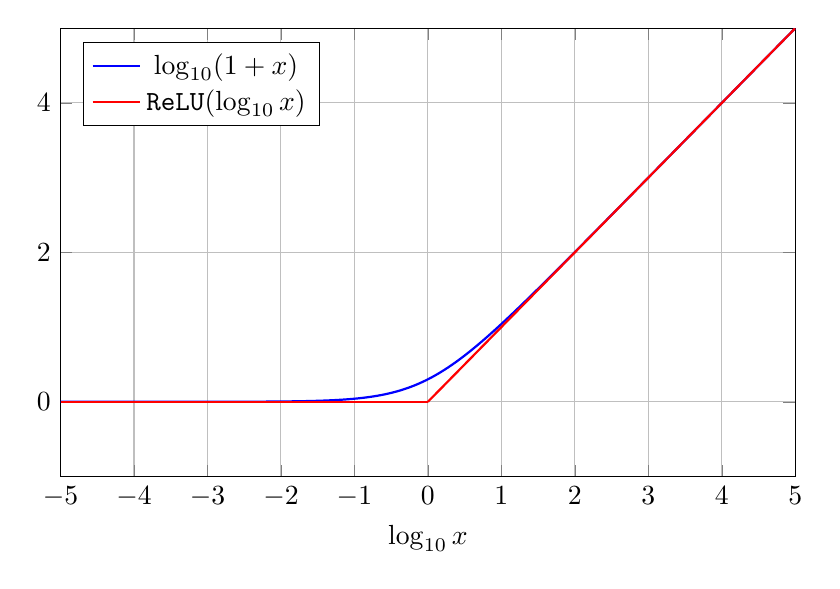
\begin{tikzpicture}
                \begin{axis}[
                    xlabel={$\log_{10} x$},
                    ylabel={},
                    legend pos=north west,
                    grid=both,
                    xmin=-5, xmax=5,
                    ymin=-1, ymax=5,
                    width=0.9\textwidth,
                    height=0.6\textwidth,
                ]
                % Plot log(1+10^x)
                \addplot[blue, thick, domain=-5:5, samples=200] {ln(1+10^x)/ln(10)};
                \addlegendentry{$\log_{10}(1+x)$}
                
                % Plot ReLU(log x) = max(0, log x)
                \addplot[red, thick, domain=-5:0, samples=50] {0};
                \addplot[red, thick, domain=0:5, samples=50] {x};
                \addlegendentry{$\mathtt{ReLU}(\log_{10} x)$}
                \end{axis}
            \end{tikzpicture}
        \end{figure}
        \end{columns}
    \end{frame}
    \begin{frame}{伯特图的绘制}
        伯特图的绘制几乎属于必考题型,也是比较简单和套路的一种考题。主要分为两个步骤:
        \uncover<2->{
            \begin{block}{第一步:求传函并因式分解}
                求出有理式形式的传递函数:$H_0\Rightarrow$幅频曲线最大值
                $$
                H(j\omega)=
                    H_0\frac{(1\pm j\frac{\omega}{\omega_{z1}})(1\pm j\frac{\omega}{\omega_{z2}})\cdots}{(1+j\frac{\omega}{\omega_{p1}})(1+j\frac{\omega}{\omega_{p2}})\cdots}
                $$
            \end{block}
        }
        \uncover<3->{
            \begin{block}{第二步: 零极点按照大小排序}
                \begin{itemize}
                    \item<4-> \textbf{幅频}\quad 碰到极点(斜率\texttt{+=})$-20\mathrm{dB/dec}$,碰到零点(斜率\texttt{+=}) $+20\mathrm{dB/dec}$。
                    \item <5-> \textbf{相频}\quad 极点滞后(相位在$0.1\sim10$倍频率内线性\textcolor{red}{\textbf{减少}})$90^\circ$,零点看左右,左\textcolor{red}{\textbf{超}}右\textcolor{red}{\textbf{滞}}$90^\circ$。
                \end{itemize}
                \end{block}
        }
    \end{frame}
    \begin{frame}{伯特图的绘制}
        以上对于没有$0$零点的情况。如果有$0$零点怎么办?
        
        \pause

        有$0$零点时,传递函数形式为
        $$
        H(j\omega)=H_0\frac{(j\frac{\omega}{\omega_{z0}})^{m}(1\pm j\frac{\omega}{\omega_{z1}})(1\pm j\frac{\omega}{\omega_{z2}})\cdots}{(1+j\frac{\omega}{\omega_{p1}})(1+j\frac{\omega}{\omega_{p2}})\cdots}
        $$
        \pause
        
        由于频率取对数后,$0$零点对应到$-\infty$,因此幅频率曲线“天生”带一个$+m\times 20\mathrm{dB/dec}$的斜率,且相频曲线“天生”带相位$m\times 90^\circ$。

        \pause

        而回到之前的公式:
        \resizebox{1\textwidth}{!}{%
        $\displaystyle
        20\log\left|H(j\omega)\right|=20\log|H_0|+\sum_{i\in\text{零点}} 20\mathtt{Relu}\left(\log\frac{\omega}{\omega_{zi}}\right)-\sum_{i\in\text{极点}} 20\mathtt{Relu}\left(\log\frac{\omega}{\omega_{pi}}\right)\textcolor{red}{+20m\log\frac{\omega}{\omega_{z0}}}
        $}

        \pause

        可见,$0$零点对$\omega_{z0}$点的增益贡献恰好为$0\mathrm{dB}$。因此只需要巧妙地把$\omega_{z0}$放进通带即可。
    \end{frame}
\end{document}